\begin{figure}[tbp]
\centering
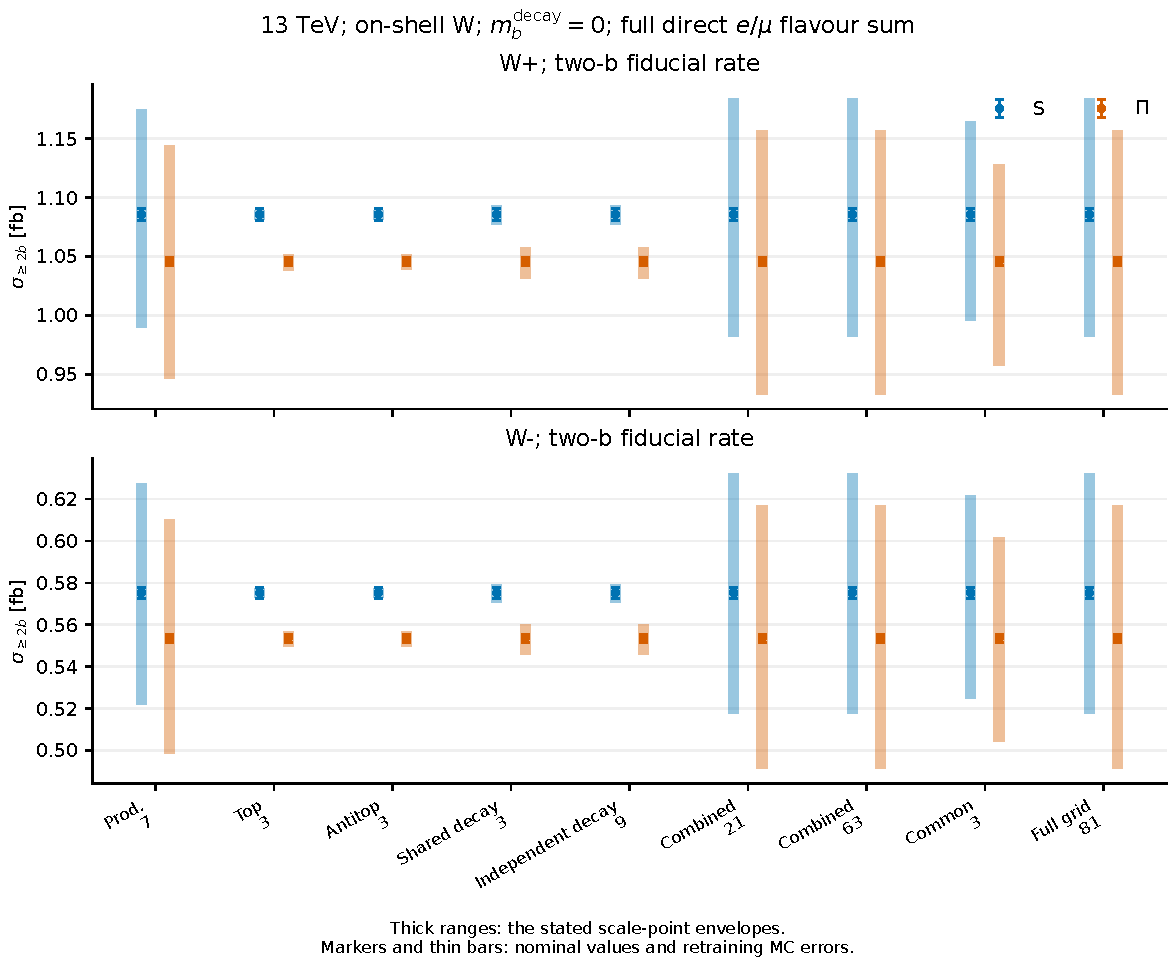
\includegraphics[width=.95\linewidth]{../figures/main_onshell_v3_coarse_v1/figure_2_scales.pdf}
\caption{Two-b fiducial cross sections for both charges. Thick intervals
show the stated production, decay and combined scale envelopes; thin bars
show independent-retraining Monte Carlo errors on the nominal predictions.
The full 81-point envelope is a diagnostic; the main envelope uses 63
points. The intervals describe scale response and are not confidence intervals.}
\label{fig:mainscales}
\end{figure}

\begin{figure}[tbp]
\centering
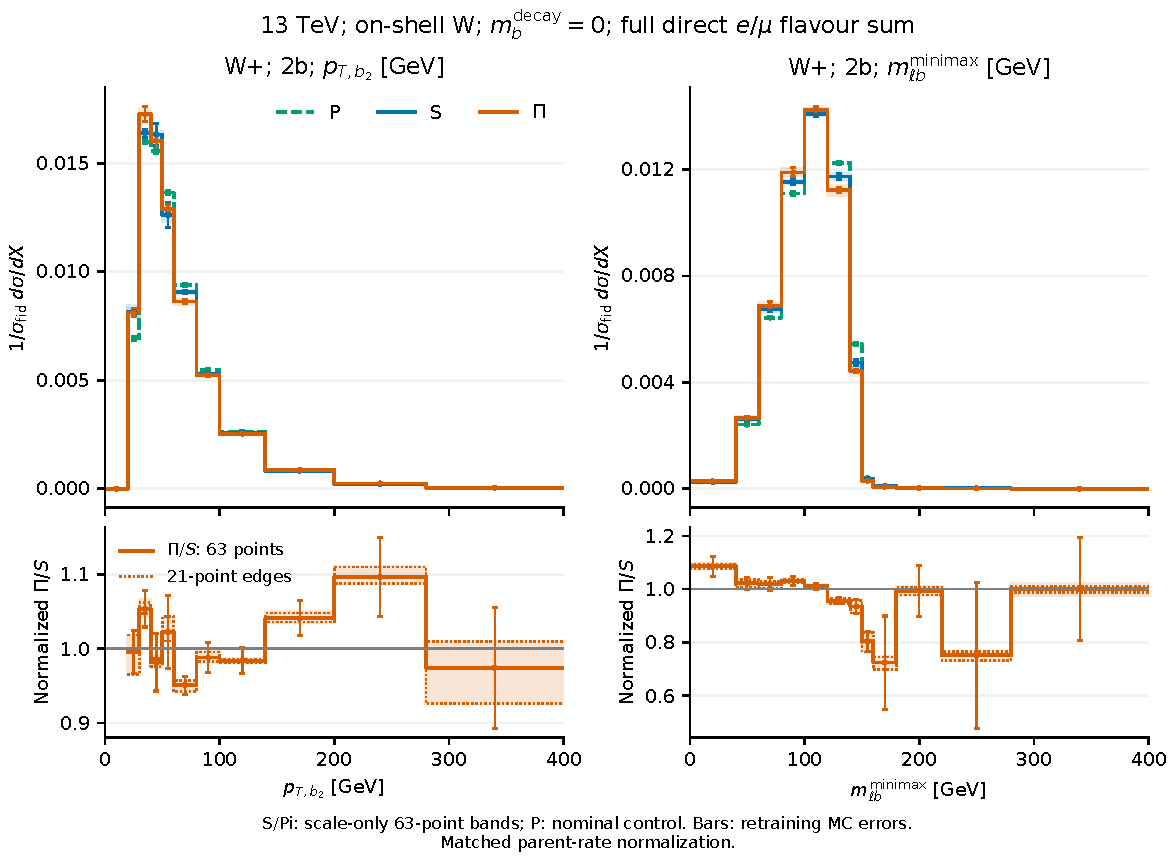
\includegraphics[width=\linewidth]{../figures/main_onshell_v3_coarse_v1/figure_3_decay.pdf}
\caption{Normalized W$^+$ two-b distributions in subleading-b transverse
momentum and $m_{b\ell}^{\rm minimax}$. The lower panels show the ratio of
the separately normalized product and strict-NLO spectra. Filled bands
use 63 matched scale points; dotted boundaries show the 21-point envelope.
Monte Carlo bars include bin--normalization covariance. The common draft
bins retain the full original range, including unresolved tails; they do
not imply uniform precision or a final choice of publication bins.}
\label{fig:maindecay}
\end{figure}

\begin{figure}[tbp]
\centering
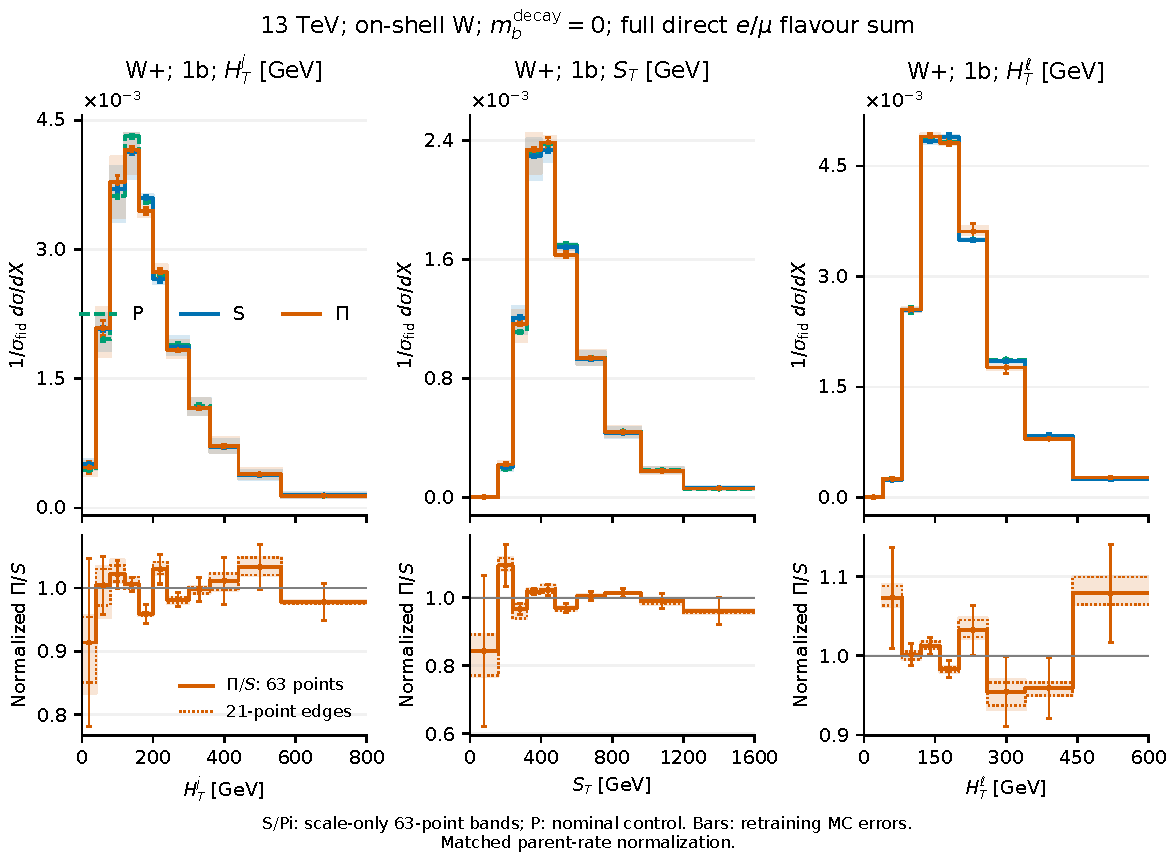
\includegraphics[width=\linewidth]{../figures/main_onshell_v3_coarse_v1/figure_4_activity.pdf}
\caption{Normalized jet $H_T$, $S_T$ and lepton $H_T$ distributions in
the W$^+$ one-b region. Conventions are those of Figure~\ref{fig:maindecay}.
Normalization uses the full corresponding fiducial rate, rather than the
sum of displayed bins; unmeasured continuous overflows are not folded in.}
\label{fig:mainactivity}
\end{figure}

\begin{figure}[tbp]
\centering
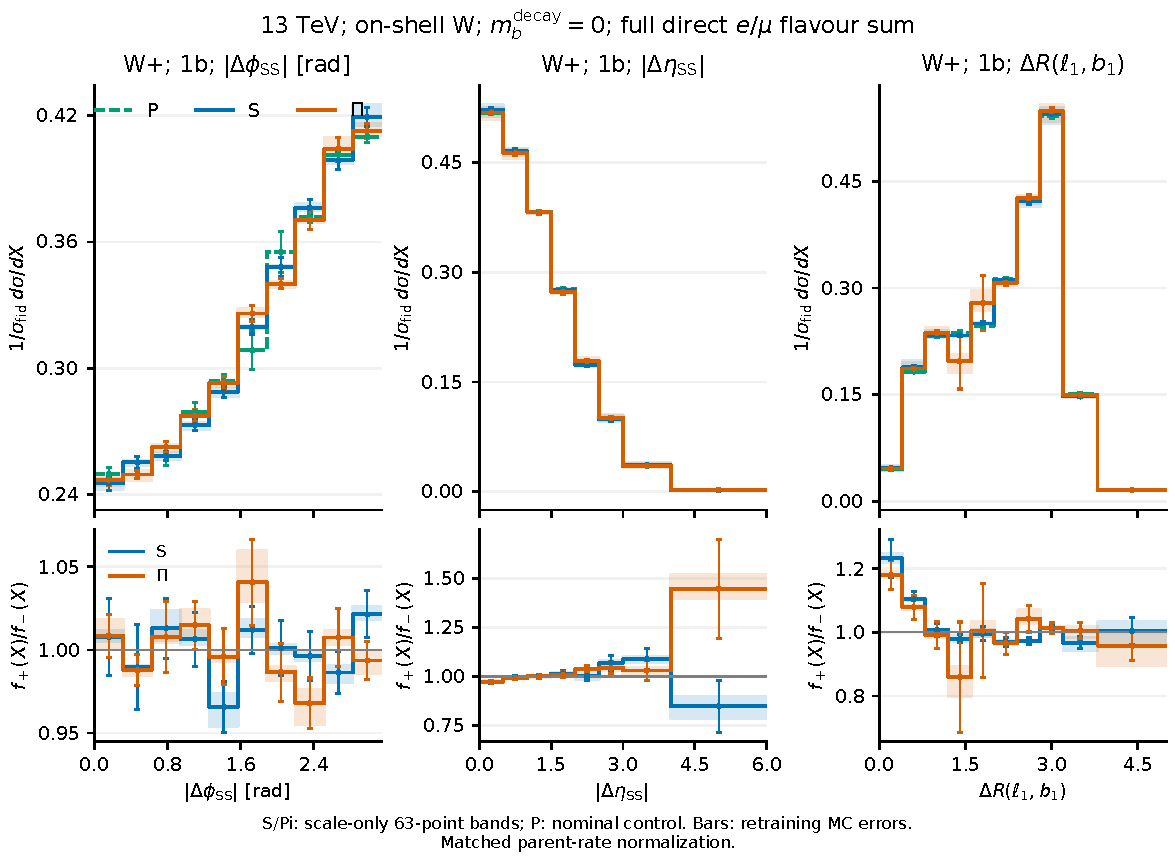
\includegraphics[width=\linewidth]{../figures/main_onshell_v3_coarse_v1/figure_5_angles_charge.pdf}
\caption{Same-sign lepton angular separations and the separation of
the leading lepton and b jet. Upper panels show normalized W$^+$ spectra.
Lower panels compare normalized W$^+$ and W$^-$ shapes for S and $\Pi$;
these are distinct from absolute differential charge ratios. Bands and
Monte Carlo bars preserve the matched scale and normalization conventions.}
\label{fig:mainangles}
\end{figure}

\begin{figure}[tbp]
\centering
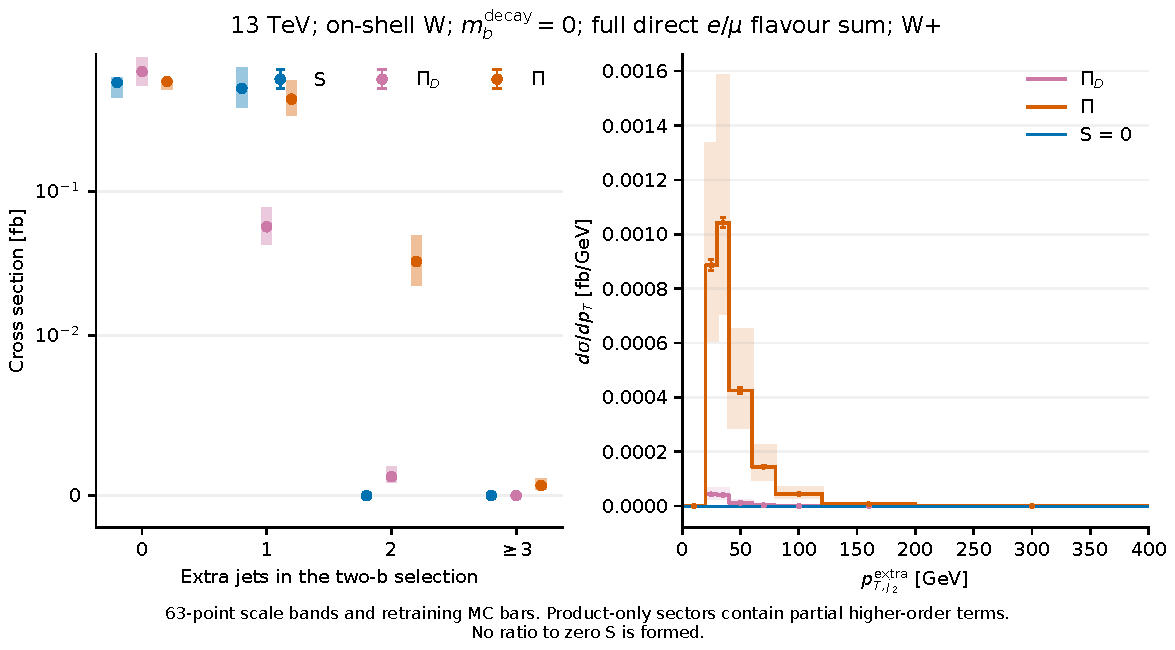
\includegraphics[width=\linewidth]{../figures/main_onshell_v3_coarse_v1/figure_6_extra_jets.pdf}
\caption{W$^+$ rates by extra-jet multiplicity in the two-b region and
the absolute second-extra-jet spectrum. The product includes emissions
from different stages, with the accuracy limitations in
Table~\ref{tab:jets}. No ratio to the vanishing strict-NLO prediction is
formed for the product-only sectors. Filled ranges are 63-point scale
envelopes and thin bars are retraining Monte Carlo errors.}
\label{fig:mainjets}
\end{figure}

\begin{figure}[tbp]
\centering
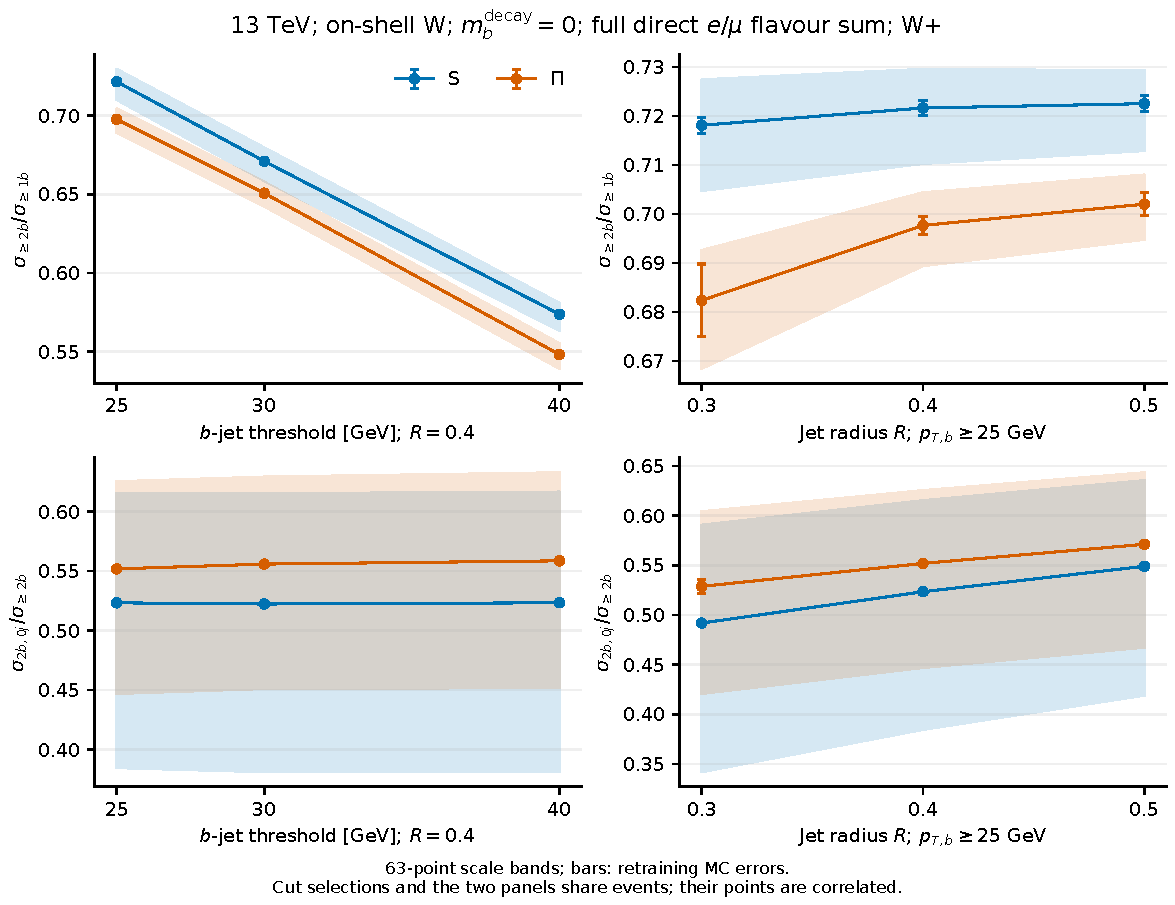
\includegraphics[width=.95\linewidth]{../figures/main_onshell_v3_coarse_v1/figure_7_migrations.pdf}
\caption{Two-b-given-one-b efficiency and the zero-extra-jet fraction
for W$^+$, versus the b-jet threshold and jet radius. All cut selections
are evaluated in the same integrations and their points are correlated.
The light-jet threshold remains at 25 GeV. Bands show 63-point scale
envelopes; bars show retraining Monte Carlo errors.}
\label{fig:mainmigrations}
\end{figure}
